\section{Spatial4D-Bench}
\label{sibench}


\subsection{Overview}
\label{sibench_overview}
Spatial4D-Bench is a large-scale, multi-task 4D spatial intelligence benchmark designed to assess the 4D spatial intelligence of MLLMs.
We name this benchmark ``Spatial4D-Bench'' as it is constructed from a large amount of video data grounded in 4D space and aims to evaluate the gap between MLLMs and human-level 4D spatial intelligence.
Spatial4D-Bench consists of \textasciitilde40,000 carefully curated and annotated QA pairs of 18 tasks, ranging from fundamental perception to complex reasoning. A detailed categorization of the 18 tasks is shown in \cref{fig_spatial4dbench_overview}.%

To ensure a comprehensive evaluation, Spatial4D-Bench aggregates data from a wide variety of publicly available datasets, encompassing both indoor and outdoor environments.
These datasets capture a rich variety of objects, actions, and scenes viewed from both egocentric and allocentric perspectives.
Instead of merely aggregating existing labels, we generate novel QA pairs across multiple datasets to maximize task diversity. 
Crucially, adhering to human spatial cognition principles~\cite{waller2013handbook, newcombe2004spatial}, we organize these 18 tasks into a hierarchical taxonomy composed of 6 core categories: \textit{object understanding}, \textit{scene understanding}, \textit{spatial relationship understanding}, \textit{spatiotemporal relationship understanding}, \textit{spatial
reasoning} and \textit{spatiotemporal reasoning}.
Compared to existing benchmarks, Spatial4D-Bench provides a more comprehensive evaluation suite to assess the spatial cognitive abilities of MLLMs, spanning a variety of tasks that parallel the versatility of human spatial intelligence. 





\subsection{Benchmark Construction}
\label{subsec:construction}

\cref{benchmark_construction_diagr_v1} illustrates an overview of the pipeline used to construct Spatial4D-Bench.
It can be seen that there are four stages in the construction pipeline, including data collection, data unification, QA pairs generation, and final human review.


\begin{figure} 
	\centering	
		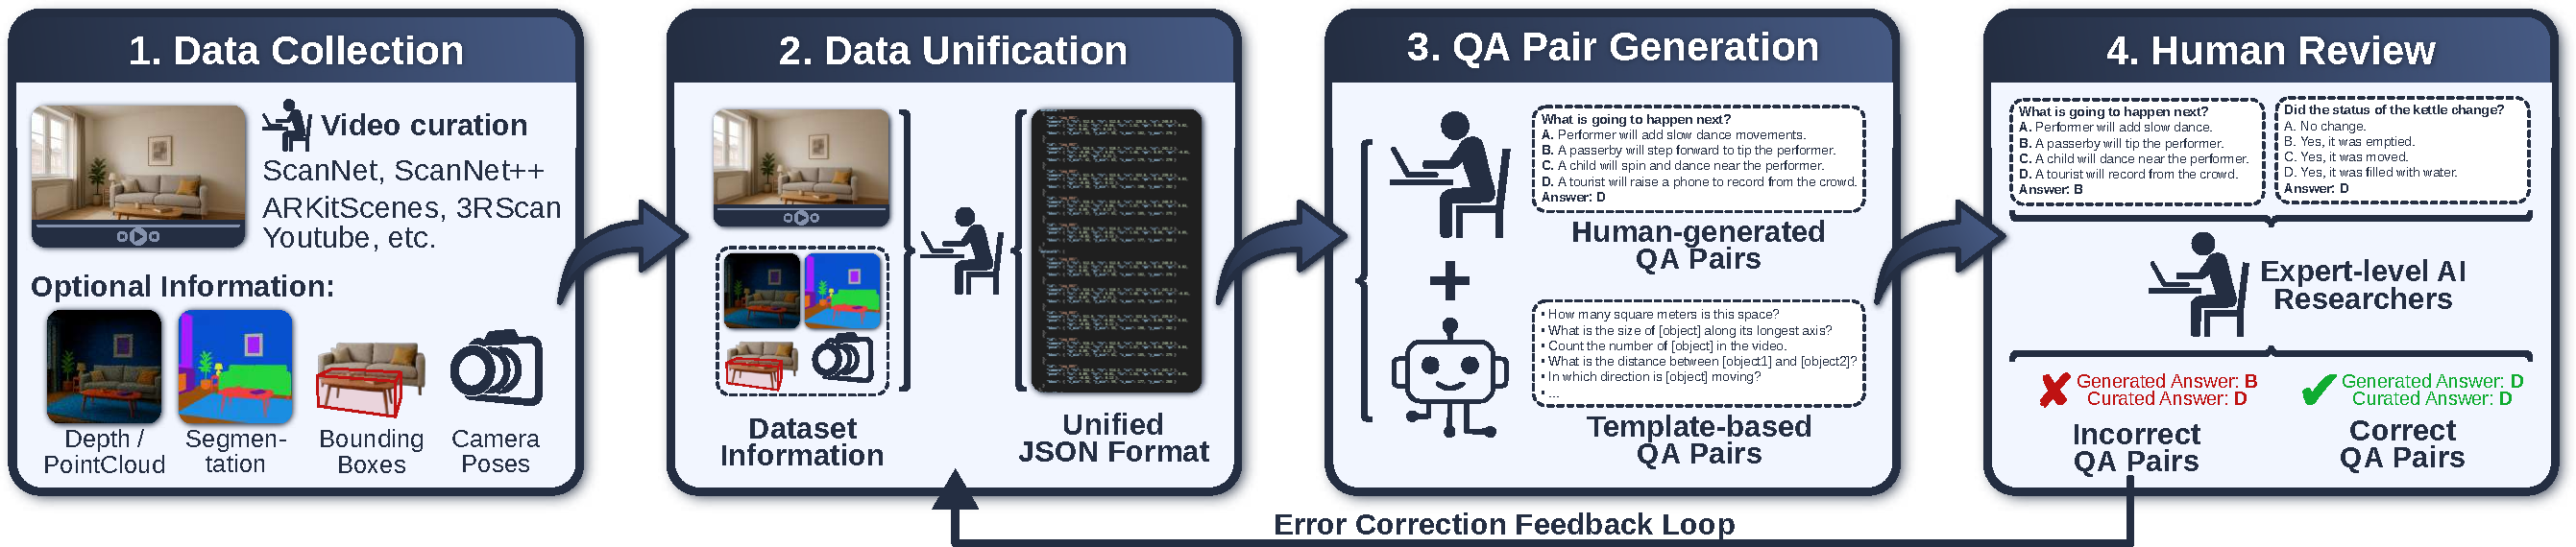
\includegraphics[width=0.99\linewidth]{Figures/data_pipeline_compressed.pdf}
	\caption{The Spatial4D-Bench construction pipeline. We unify diverse data sources into a standardized metadata format, generating QA pairs via templates and expert annotation, followed by rigorous human verification.   
	\label{benchmark_construction_diagr_v1} }
\end{figure}




\paragraph{Data Collection.}
In the first stage, we collect a large amount of data from a variety of datasets, including Charades-Ego~\cite{sigurdsson2018charades}, ARKitScenes~\cite{baruch2021arkitscenes}, ScanNet~\cite{dai2017scannet}, ScanNet++~\cite{yeshwanth2023scannet++}, 3RScan~\cite{wald2019rio}, RoomTour3d~\cite{han2025roomtour3d}, EPIC-KITCHENS~\cite{Damen2018EPICKITCHENS}, ADL~\cite{youhome2022}, EgoTaskQA~\cite{jia2022egotaskqa}, HoloAssist~\cite{wang2023holoassist}, IndustReal~\cite{schoonbeek2024industreal}, YouCook2~\cite{zhou2018towards}, Video-MME~\cite{fu2024video},
VideoPhy-2~\cite{bansal2025videophy}, and nuScenes~\cite{caesar2020nuscenes}.
These datasets encompass various objects, actions, and scenes across indoor and outdoor scenarios, egocentric and allocentric perspectives, and both real and synthetic/generated data, contributing to the diversity and comprehensiveness of Spatial4D-Bench.
We aggregate diverse data modalities from the participating datasets, including text, RGB videos, and point clouds (used only to facilitate QA annotation).
\cref{fig:dataset_statistics} summarizes the source datasets that contribute to each task in Spatial4D-Bench.
In addition, as shown in~\cref{benchmark_construction_diagr_v1}, this stage includes a human verification loop to filter out low-quality scans or incomplete annotations, ensuring that the input data meet the reliability requirements.



\paragraph{Data Unification.}
In the second stage, we convert the collected data into a unified metadata structure following~\cite{Yang_2025_CVPR} since these data are collected from a variety of datasets and are heterogeneous.
This standardization facilitates consistent downstream task generation and enables traceability for error correction during human review and verification.
During this stage, we also preprocess image frames, sourced from RoomTour3D~\cite{han2025roomtour3d}, for the \textit{route plan} task by tagging room names on the relevant frames.
This preprocessing disambiguates the route planning targets, ensuring that the model focuses on spatial planning capabilities rather than OCR capabilities. For \textit{action prediction} and \textit{spatial memory} tasks, we select and extract video clips with various lengths from EPIC-KITCHENS~\cite{Damen2018EPICKITCHENS}, ADL~\cite{youhome2022}, EgoTaskQA~\cite{jia2022egotaskqa}, HoloAssist~\cite{wang2023holoassist}, IndustReal~\cite{schoonbeek2024industreal}, and Video-MME~\cite{fu2024video}, to satisfy the particular design requiremets of the QA pairs, achieving consistency between a QA pair and its corresponding video clip in the context of the given tasks. As a result, a subset of videos from the above-mentioned datasets have been preprocessed in curating Spatial4D-Bench.
Human review and verification are also used in this stage to ensure the correctness of data unification.



\paragraph{QA Pairs Generation.}
With the standardized metadata, we generate Question-Answer (QA) pairs via a combination of human annotation and automatic template-based generation.
We recruit several well-educated annotators with relevant backgrounds to design QA pairs for tasks including \textit{object attribute estimation, spatial memory, state change detection, egocentric reasoning, route plan, action prediction, and physical plausibility reasoning}.
Most of these tasks involve complex spatiotemporal understanding and reasoning in high-level cognition, making automatic template-based generation prone to producing low-quality QA pairs, whereas human annotation produces significantly higher-quality ones.
For the other tasks, we use automatic template-based generation based on well-designed template and ground-truth labels.
Specifically, for tasks involving rigid geometric properties, such as object counts, dimensions, and distances, we utilize template-based generation derived from the unified metadata.
And for tasks involving 3D boxes and coordinate systems, we provide multiple instruction formats such as object 3D bounding boxes, text descriptions of objects/rooms, or a combination of both, allowing foundation models to be tested with diverse instruction types.
Note that templates are also provided for annotating egocentric reasoning to assist human annotators.
Throughout this stage, humans continuously review and verify the generated QA pairs to judge, refine, correct, and filter out incorrect and ambiguous questions, options, and answers.


\begin{figure}
    \centering
    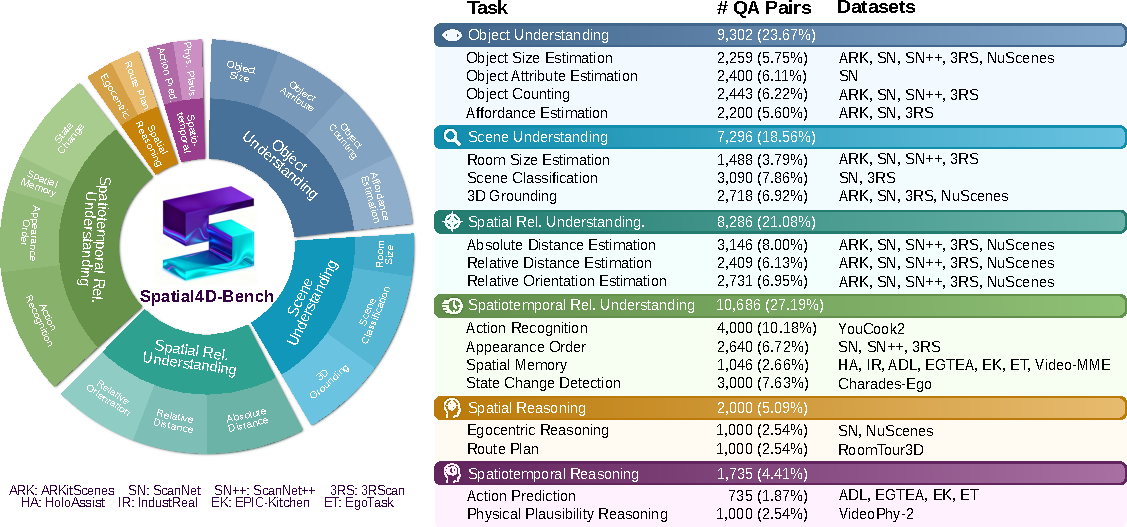
\includegraphics[width=0.99\linewidth]{Figures/dataset_statistics_v2.pdf}
    \caption{Distribution of question-answer pairs provided by our Spatial4D-Bench.}
    \label{fig:dataset_statistics}
\end{figure}


\paragraph{Final Human Review.}
In the final stage, experienced AI researchers perform the final human review to filter out ambiguous or incorrect QA pairs, \eg, checking whether a textual description uniquely identifies a target object.
As illustrated in \cref{benchmark_construction_diagr_v1}, errors detected at this stage will trigger a feedback loop where issues are traced back to the source metadata for correction.
Finally, we select \textasciitilde40,000 high-quality QA pairs to construct the Spatial4D-Bench.
Some examples of QA pairs can be found in the appendix (\cref{tab:example_qas_table_1} and \cref{tab:example_qas_table_2}).






\subsection{Task Taxonomy}
\label{subsec:taxonomy}

To systematically evaluate the gap between current MLLMs and human-level spatial cognition, as shown in \cref{fig:spatial_cogn_diagram}, we organize the 18 tasks into a hierarchical taxonomy composed of six core categories: \textit{object understanding}, \textit{scene understanding}, \textit{spatial relationship understanding}, \textit{spatiotemporal relationship understanding}, \textit{spatial reasoning} and \textit{spatiotemporal reasoning}. This taxonomy progresses from object/scene-level perception, through spatial/spatiotemporal understanding, to dynamic spatial/spatiotemporal reasoning, mirroring the cognitive abilities of human intelligence~\cite{waller2013handbook, newcombe2004spatial}.


\paragraph{Object Understanding.} Spatial intelligence begins with the accurate perception of intrinsic physical properties, which is a prerequisite for interacting with a physical scene.
This category includes \textit{object size estimation}, \textit{object attribute estimation},  \textit{object counting} and \textit{affordance estimation}. 
A robust spatial agent must ground visual features into both precise metric values (size) and semantic properties (attributes).
While existing benchmarks such as VSI-Bench~\cite{Yang_2025_CVPR} evaluate metric properties, they often overlook intrinsic attributes such as color, shape, and material.
Spatial4D-Bench integrates both metric and attribute understanding into a unified evaluation framework.
Crucially, we also incorporate \textit{affordance estimation} here as a functional attribute. 
Unlike SIBench~\cite{yu2025far} or SpaCE-10~\cite{gong2025space}, which focus on simple existence queries (\eg, ``is there an item to sit on?''), we integrate affordance with 3D grounding, requiring the model to identify the specific spatial position that satisfies a functional description (\eg, ``which position allows me to wash hands?''). 
This verifies that MLLMs possess a comprehensive understanding of an object's physical characteristics, which is a fundamental prerequisite for complex interaction tasks.


\paragraph{Scene Understanding.} Beyond isolated entities, an agent must comprehend the global semantic and geometric context of the environment to answer ``what'' is present and ``where'' it belongs.
This category encompasses \textit{room size estimation}, \textit{scene classification}, and \textit{3D grounding}.
Here, the model must abstract local visual cues into a broader understanding of the environment type and its volumetric scale.
Crucially, we include \textit{3D grounding} (object detection and localization in 3D space) in this category as it represents the population of the scene layout.
Unlike benchmarks like InternSpatial~\cite{deng2025internspatial} that rely on 2D bounding boxes, our \textit{3D grounding} task requires 3D spatial grounding, ensuring that MLLMs possess a volumetric understanding of object placement. 



\paragraph{Spatial Relationship Understanding.} Once entities and the scene are defined, a spatial intelligence model needs to be able to resolve the geometric topology and metric layout between them.
This category is composed of \textit{relative distance estimation}, \textit{absolute distance estimation} and \textit{relative orientation estimation}.
Navigating the physical world requires resolving spatial ambiguities. By evaluating both relative (topological) and absolute (metric) distances, we test the robustness of the model's depth perception.
While benchmarks like SpatialRGPT~\cite{cheng2024spatialrgpt} address relative spatial relations, we enforce a more strict evaluation by combining relative topology with absolute metric estimation, ensuring that the model is not merely guessing based on 2D perspective cues.

\paragraph{Spatiotemporal Relationship Understanding.} Incorporating the fourth  dimension of time, this category evaluates the ability to track object states and dynamics over time. This category represents the leap from 3D to \textbf{4D spatial intelligence}.
Tasks include \textit{action recognition}, \textit{appearance order}, \textit{spatial memory}, and \textit{state change detection}.
The real world is a dynamic environment in which spatial and temporal aspects continuously evolve, and humans living in such an environment inherently develop 4D spatial intelligence that supports a wide range of spatial understanding and reasoning abilities.
While VSI-Bench includes basic appearance ordering~\cite{Yang_2025_CVPR} where clearly visible objects need to be identified in terms of the sequence in which they show up in a video, true 4D intelligence requires maintaining a coherent world model of objects even when they are occluded.
Our \textit{spatial memory} task evaluates this working memory capability by requiring the models to track objects that exit the field of view.
\textit{Action recognition} evaluates the model's ability to semantically categorize dynamic events within 3D space, bridging the gap between object detection and dynamic scene understanding.
Furthermore, \textit{state change detection} tests the causal understanding of interactions over time, such as a door opening rather than just movement tracking, distinguishing between simple movement and meaningful state transitions (e.g., a door opening).



\begin{figure} 
	\centering	
		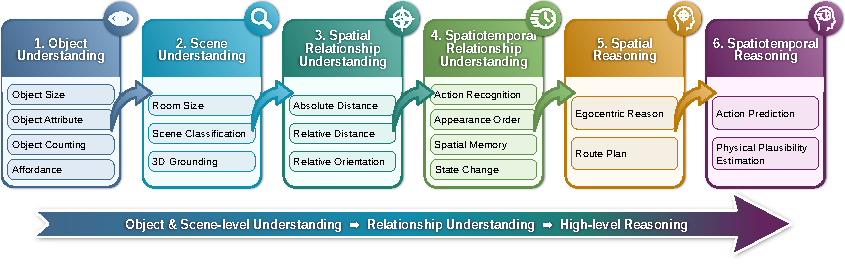
\includegraphics[width=0.99\linewidth]{Figures/taxonomy_v2.pdf} 
    \caption{Spatial4D-Bench Task Taxonomy.
    We organize 18 distinct tasks into 6 progressive categories representing the spectrum of spatial cognition.
    The taxonomy progresses from perception and understanding in object/scene level, through spatial/spatiotemporal understanding, to dynamic spatial/spatiotemporal reasoning, mirroring the cognitive abilities of human intelligence.}
     \label{fig:spatial_cogn_diagram}
\end{figure}

\paragraph{Spatial Reasoning.} Moving from passive perception to active embodiment, this category assesses the agent's ability to reason about its own state and plan movements.
It is composed of \textit{egocentric reasoning} and \textit{route plan}.
We introduce \textit{egocentric reasoning} to challenge the model to infer the observer's own spatial state (\eg, ``how did the camera rotate?''), which is a prerequisite for self-localization.
This capability is critical for embodied agents operating in first-person views to localize themselves within the environment, moving beyond purely allocentric reasoning.
Building on this, our \textit{route plan} task elevates the difficulty beyond the single-room queries of VSI-Bench~\cite{Yang_2025_CVPR}.
Instead of using single-room single-step queries found in previous benchmarks~\cite{Yang_2025_CVPR}, we require long-horizon trajectory planning across multiple rooms, simulating the sequential cognitive load of a mobile robot operating in a complex environment.
To answer correctly, the model must predict a valid \textit{sequence} of actions (\eg, selecting the correct directions for multiple blanks in an instruction set) rather than a single directional move.

\paragraph{Spatiotemporal Reasoning.}
The highest level of spatial cognition involves abstracting perceptual data into predictive models and physical laws.
Tasks include \textit{action prediction} and \textit{physical plausibility reasoning}.
True spatial intelligence implies a ``world model'' that allows for prediction and physical intuition, capabilities largely ignored by existing benchmarks listed in \cref{tab:recent_mllm_eval_benchmarks}.
\textit{Action prediction} evaluates this capability by demanding that the model forecasts future events based on partial visual history.
Unlike understanding tasks that rely on retrospective classification, prediction requires causal inference: the model must synthesize observed dynamics with logical deduction to anticipate the likely intent of agents or the physical trajectory of objects.
Complementing this, \textit{physical plausibility reasoning} (using AI-generated videos of physical anomalies) tests whether the model has internalized the laws of physics, allowing it to identify violations of physical laws (\eg, gravity defiance), ensuring that their reasoning is grounded in reality.
This category benchmarks the transition from passive perception to active reasoning.
